\chapter{Tang}\label{tang} \todo{re-factor entire chapter}

Automated decryption of HDDs with Tang blablebli.

Before Tang, automated decryption was usually handled by a Key Escrow server.

\section{Key Escrow}\label{escrow}

The Key Escrow server (also known as a “fair” cryptosystem) is providing escrow service for encryption keys.
A client using Key Escrow usually generates a key, encrypts data with it and then stores the key encryption key on a remote server.
Unfortunatelly, it is not always as simple as it sounds and there are couple of security concerns.

To transfer the encryption keys we want to store on an Escrow server, we have to encrypt the channel on which we send them.
When transmitting keys over an insecure network without an encrypted link, anyone listening to the network traffic could immadiately fetch the key.
This should signal security risks, and, of course, we do not want any third party to access our secret data.
Usually we encrypt a channel with TLS(Transport Layer Security) or GSSAPI (Generic Security Services Application Program Interface) as shown on a Figure \ref{fig:escrowmodel} Escrow model.
\begin{figure}[h]
    \centering
    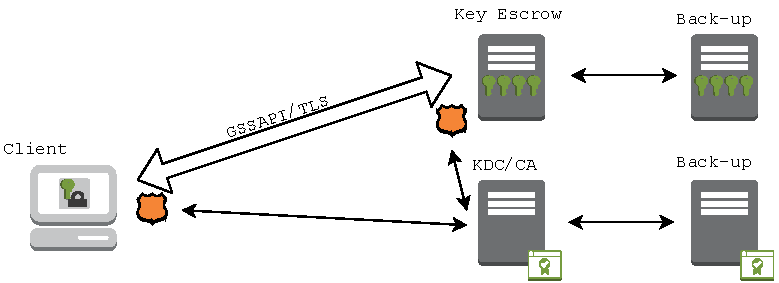
\includegraphics[scale=0.7]{figures/EscrowModel.pdf}
    \caption{Escrow model}
    \label{fig:escrowmodel}
\end{figure}
Unfortunatelly, this is not enough to have the communication secure.
We can not just start sending these keys to the escrow server if we do not know whether this server is the one it acts to be.
This server has to have its identity verified, and the client has to authenticate to this server too.
The increasing amount of keys implicates a need for Certification Authority server (CA) or a Key Distribution Center (KDC) to manage all of them.

With all these keys, and at this point only, server can verify if the client is permitted to get their key, and the client is able to identify trusted server.
This is a fully stateful process.
To sum up, an authorized third party may gain access to keys stored on an Escrow server under certain circumstances only.

The complexity of this system increases the attack surface and for a such complex system it would be unimaginable not to have backups.
Escrow server may store lots of keys from lots of different places, users and services.

With key escrow a third party gets copies of a cryptographic key.
People might not be comfortable with any third party having this ability and that "technical" problems vex the key escrow solution.
Tang's key recovery, on the other hand, lets us just "backup" and restore cryptographic keys anonymously and without any third party possesing our key.

Key recovery is necessary.
Key escrow is not.
Let us not confuse these two.

\section{Tang - binding daemon}

Tang server is an open source project implemented in C programming language, and it binds data to network presence.
What does binding data to network presence really mean? \todo{do not ask}
Essentially, it allows us to make some data to be available only when the system containing the data is on a particular, usually secure, network.

Tang server advertises asymmetric keys and a client is able to get the list of these signing keys \ref{jose} by HTTP (Hypertext Transfer Protocol) GET request.
The next step is the provisioning step. With the list of these public keys the process of encrypting data may start.
A client chooses one of the asymmetric keys to generate a unique encryption key.
After this, the client encrypts data using the created key. Once the data is encrypted, the key is discarded.
Some small metadata have to be produced as a part of this operation. The client should store these metadata to work with it when decrypting.

Finally, when the client wants to access the encrypted data, it must be able to recover encryption key.
This step starts with loading the stored metadata and ends with simply performing a HTTP POST to Tang server.
Server performs its mathematical operation and sends the result back to the client.
Finally, the client has to calculate the key value, which is better than when server calculates it.
So the Tang server never knew the value of the key and literraly nothing about its clients.

\begin{figure}[h]
    \centering
    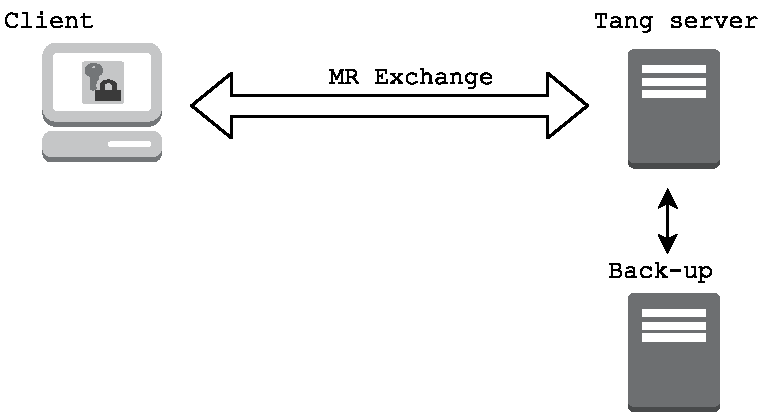
\includegraphics[scale=0.7]{figures/TangModel.pdf}
    \caption{Tang model}
    \label{fig:tangmodel}
\end{figure}

On Figure \ref{fig:tangmodel} you can see the Tang model.
It is very similar to Escrow model \ref{fig:escrowmodel} but there are some thing missing.
In fact, there is no longer a need for TLS channel to secure comunication between the client and the server,
 and that is the reason why Tang implements the McCallum-Relyea exchange \ref{mrexchange} as described below.

\section{Binding with Tang}

A client performs an ECDH key exchange using the McCallum-Relyea algorithm \ref{mrexchange} in order to generate the binding key.
Then the client discards its own private key so that the Tang server is the only party that can reconstitute the binding key.
To blind \todo{blind?} the client's public key and the binding key, Tang uses a third, ephemeral key.
Ephemeral key is generated for each execution of a key establishment process.
Now only the client can unblind his public key and binding key.

\begin{table}[h]
\centering
\label{mrexchange}
\begin{tabular}{c|c|c|c}
\hline
\multicolumn{2}{c|}{Provisioning} & \multicolumn{2}{c}{Recovery} \\ \hline  used
client's side & server's side & client's side & server's side \\ \hline
 & $ S \epsilon _{R} [1, p-1]$ & $E \epsilon _{R} [1, p-1]$ &  \\
 & $s = gS$ &$ x = c + gE$ &  \\
 & $\leftarrow$  s &  x $\rightarrow$ &  \\
$C \epsilon _{R} [1, p-1]$ &  &  & $y = zS $\\
$e = gC $&  &  & $\leftarrow$ y \\
$K = gSC = sC$ &  & $K = y - sE $&  \\
Discard: K, C &  &  &  \\
Retain s, c &  &  &  \\ \hline
\end{tabular}
\caption{McCallum-Relyea exchange}
\end{table}

\section{Provisioning}
The client selects one of the Tang server's exchange keys (we will call it sJWK; identified by the use of deriveKey in the sJWK's key\_ops attribute).
The lowercase "s" stands for server's key pair and JWK is used format of the message.
The client generates a new (random) JWK (cJWK; c stands for client's key pair).
The client performs its half of a standard ECDH exchange producing dJWK which it uses to encrypt the data.
Afterwards, it discards dJWK and the private key from cJWK.

The client then stores cJWK for later use in the recovery step.
Generally speaking, the client may also store other data, such as the URL of the Tang server or the trusted advertisement signing keys.

\begin{equation}
    s = g * S
\end{equation}

\begin{equation}
    c = g * C
\end{equation}

\begin{equation}
    K = s * C
\end{equation}

\section{Recovery}
To recover dJWK after discarding it, the client generates a third ephemeral key (eJWK).
Using eJWK, the client performs elliptic curve group addition of eJWK and cJWK, producing xJWK. The client POSTs xJWK to the server.

The server then performs its half of the ECDH key exchange using xJWK and sJWK, producing yJWK. The server returns yJWK to the client.

The client then performs half of an ECDH key exchange between eJWK and sJWK, producing zJWK. Subtracing zJWK from yJWK produces dJWK again.

Mathematically (capital is private key; g stands for generate) client's operation:

\begin{equation}
    e = g * E
\end{equation}

\begin{equation}
    x = c + e
\end{equation}

\begin{equation}
    y = x * S
\end{equation}

\begin{equation}
    z = s * E
\end{equation}

\begin{equation}
    K = y - z
\end{equation}

\section{Security}

We can now compare Tang and Escrow. In contrast, Tang is stateless and doesn't require TLS or authentication.
Tang also has limited knowledge. Unlike escrows, where the server has knowledge of every key ever used, Tang never sees a single client key.
Tang never gains any identifying information from the client.

\begin{table}[h]
\centering
\label{compare}
\begin{tabular}{@{}lll@{}}
\toprule
               & Escrow   & Tang                         \\ \midrule
Stateless      & No       & Yes                          \\
SSL/TLS        & Required & Optional                     \\
X.509          & Required & Optional                     \\
Authentication & Required & Optional                     \\
Anonymous      & No       & Yes                          \\ \bottomrule
\end{tabular}
\caption{Comparing Escrow and Tang}
\end{table}

Let's think about the security of Tang system. Is it really secure without an encrypted channel or even without authentication?
So long as the client discards its private key, the client cannot recover dJWK without the Tang server.
This is fundamentally the same assumption used by Diffie-Hellman (and ECDH).

\subsection{Man-in-the-Middle attack}
In this case, the eavesdropper in this case sees the client send xJWK and receive yJWK.
Since, these packets are blinded by eJWK, only the party that can unblind these values is the client itself (since only it has eJWK's private key).
Thus, the MitM attack fails.
\subsection{Compromise the client to gain access to cJWK}
It is of utmost importance that the client protects cJWK from prying eyes.
This may include device permissions, filesystem permissions, security frameworks (such as SELinux - Security-Enhanced Linux) or even the use of hardware encryption such as a TPM.
How precisely this is accomplished depends on the client implementation.
\subsection{Compromise the server to gain access to sJWK's private key}
The Tang server must protect the private key for sJWK.
In this implementation, access is controlled by file system permissions and the service's policy.
An alternative implementation might use hardware cryptography (for example, an HSM) to protect the private key.
\section{Building Tang}

Tang is originally packaged for Fedora OS version 23 and later but we can build it from source of course.
It relies on few other software libraries:
\label{dependencies}
\begin{itemize}
\item http-parser \ref{http-parser}
\item systemd / xinetd \ref{systemd}
\item jose \ref{jose}
    \begin{itemize}
    \item jansson \ref{jansson}
    \item openssl \ref{openssl}
    \item zlib \ref{zlib}
    \end{itemize}
\end{itemize}

The steps to build it from source include download source from poject's GitHub or clone~it.
Make sure you have all needed dependencies installed and then run:
\begin{lstlisting}[columns=fixed,tabsize=4,backgroundcolor=\color{yellow!10}]
\$ autoreconf -if
\$ ./configure --prefix=/usr
\$ make
# sudo make install
\end{lstlisting}
Optionally to run tests:
\begin{lstlisting}[columns=fixed,tabsize=4,backgroundcolor=\color{yellow!10}]
\$ make check
\end{lstlisting}
\section{Server enablement}

Enabling a Tang server is a two-step process.
First, enable and start the service using systemd.
\begin{lstlisting}[columns=fixed,tabsize=4,backgroundcolor=\color{yellow!10}]
\$ sudo systemctl enable tangd-update.path --now
\end{lstlisting}
\begin{lstlisting}[columns=fixed,tabsize=4,backgroundcolor=\color{yellow!10}]
\$ sudo systemctl start tangd-update.path
\end{lstlisting}

\begin{lstlisting}[columns=fixed,tabsize=4,backgroundcolor=\color{yellow!10}]
\$ sudo systemctl enable tangd.socket --now
\end{lstlisting}


Second, generate a signing key and an exchange key.
\begin{lstlisting}[columns=fixed,tabsize=4,backgroundcolor=\color{yellow!10}]
# jose gen -t '{"alg":"ES256"}' -o /var/db/tang/sig.jwk
\end{lstlisting}

\begin{lstlisting}[columns=fixed,tabsize=4,backgroundcolor=\color{yellow!10}]
# jose gen -t '{"kty":"EC","crv":"P-256","key_ops":["deriveKey"]}' \
        -o /var/db/tang/exc.jwk
\end{lstlisting}

Now we are up and running. Server is ready to send advertisment on demand.
\todo{Get clevis in here?}


\section{Clevis client}\label{clevis}

Clevis provides a pluggable key management framework for automated decryption.
It can handle even automated unlocking of LUKS volumes.
To do so, we have to encrypt some data with simple command:

\begin{lstlisting}[columns=fixed,tabsize=4,backgroundcolor=\color{yellow!10}]
\$ clevis encrypt PIN CONFIG < PLAINTEXT > CIPHERTEXT.jwe
\end{lstlisting}

In clevis terminology, a {\it pin} is a plugin which implements automated decryption.
We simply pass the name of supported pin here.
Secondly {\it config} is a JSON object which will be passed directly to the {\it pin}.
It contains all the necessary configuration to perform encryption and setup automated decryption.

\subsection{PIN: Tang}
Clevis has full support for Tang. Here is an example of how to use Clevis with Tang:
\begin{lstlisting}[columns=fixed,tabsize=4,backgroundcolor=\color{yellow!10}]
\$ echo hi | clevis encrypt tang '{"url": "http://tangserver"}' > hi.jwe
 The advertisement is signed with the following keys:
     kWwirxc5PhkFIH0yE28nc-EvjDY

 Do you wish to trust the advertisement? [yN] y
\end{lstlisting}
In this example, we encrypt the message "hi" using the Tang pin.
The only parameter needed in this case is the URL of the Tang server.
During the encryption process, the Tang pin requests the key advertisement from the server and asks you to trust the keys.
This works similarly to SSH.

Alternatively, you can manually load the advertisment using the adv parameter.
This parameter takes either a string referencing the file where the advertisement is stored, or the JSON contents of the advertisment itself.
When the advertisment is specified manually like this, Clevis presumes that the advertisement is trusted.
\subsection{PIN: HTTP}
Clevis also ships a pin for performing escrow using HTTP.
Please note that, at this time, this pin does not provide HTTPS support and is suitable only for use over local sockets.
This provides integration with services like Custodia.

\subsection{PIN: SSS - Shamir Secret Sharing}
Clevis provides a way to mix pins together to provide sophisticated unlocking policies.
This is accomplished by using an algorithm called Shamir Secret Sharing (SSS).

\subsection{Binding LUKS volumes}
Clevis can be used to bind a LUKS volume using a pin so that it can be automatically unlocked.

How this works is rather simple. We generate a new, cryptographically strong key. This key is added to LUKS as an additional passphrase. We then encrypt this key using Clevis, and store the output JWE inside the LUKS header using LUKSMeta.

Here is an example where we bind {\tt /dev/vda2} using the Tang ping:
\begin{lstlisting}[columns=fixed,tabsize=4,backgroundcolor=\color{yellow!10}]
\$ sudo clevis bind-luks /dev/sda1 tang '{"url": "http://tang.local"}'
The advertisement is signed with the following keys:
        kWwirxc5PhkFIH0yE28nc-EvjDY

Do you wish to trust the advertisement? [yN] y
Enter existing LUKS password:
\end{lstlisting}

Upon successful completion of this binding process, the disk can be unlocked using one of the provided unlockers.

\subsection{Dracut}\label{dracut}
The Dracut unlocker attempts to automatically unlock volumes during early boot.
This permits automated root volume encryption.
Just rebuild your initramfs after installing Clevis:

\begin{lstlisting}[columns=fixed,tabsize=4,backgroundcolor=\color{yellow!10}]
\$ sudo dracut -f
\end{lstlisting}

Upon reboot, you will be prompted to unlock the volume using a password. In the background, Clevis will attempt to unlock the volume automatically. If it succeeds, the password prompt will be cancelled and boot will continue.

\subsection{UDisks2}\label{udisk2}
Our UDisks2 unlocker runs in your desktop session.
You should not need to manually enable it; just install the Clevis UDisks2 unlocker and restart your desktop session.
The unlocker should be started automatically.

This unlocker works almost exactly the same as the Dracut unlocker.
If you insert a removable storage device that has been bound with Clevis, we will attempt to unlock it automatically in parallel with a desktop password prompt.
If automatic unlocking succeeds, the password prompt will be dissmissed without user intervention.
